%%%% NB: Der Kopf sieht in dieser Tex-Datei anders aus als üblich. (PR)
\begin{Ueberlieferung}% 
{\textit{L}}Konzept: LH XXXVII 5 Bl. 202-203. 1 Bog. 2\textsuperscript{o}. 4 S. einspaltig;
der Text beginnt unver\-mittelt auf Bl. 202~r\textsuperscript{o}.
Der Bog. ist von dem aus Bl. 201 und 204 bestehenden Bog. um\-schlossen,
welcher N. ?? % F/1 = 037,05_201
und N. ?? % F/2 = 037,05_204
überliefert.
Wasserzeichen auf Bl. 203.\\
Cc 2, Nr. 967 B 
\end{Ueberlieferung}
\vspace*{8mm}
\begin{Datierungsgruende}%
Das vorliegende Stück N. ?? % F/3 = 037,05_202-203
beginnt mit der wörtlichen lateinischen Übersetzung eines Beweisgangs zur Bruchfestigkeit von Balken, den Galilei\protect\index{Namensregister}{\textso{Galilei} (Galilaeus, Galileus), Galileo 1564-1642} im zweiten Dialog seiner \textit{Discorsi e dimostrazioni matematiche} anführt.
Leibniz kommentiert den Beweisgang Schritt für Schritt und äußert anschließend eine ausführliche Kritik darüber.
Diese letzere entspricht der Kritik, die er in N. ?? % F/1 = 037,05_201
über dieselbe Stelle aus Galileis \textit{Discorsi} zum Ausdruck bringt (siehe oben, S. \pageref{037,05_201}ff.). 
Hiermit weist das vorliegende Stück einen unmittelbaren inhalt\-lichen Zusammenhang mit N. ?? % F/1 = 037,05_201 
auf. Im Textträger von N. ?? % F/3 = 037,05_202-203
findet sich ferner das gleiche Wasserzeichen wie auf Bl. 201,
auf dem N. ?? % F/1 = 037,05_201
überliefert ist.
Aus diesen Gründen wird die für N. ?? % F/1 = 037,05_201
vorgeschlagene Datierung auch für das vorliegende Stück übernommen. 
\end{Datierungsgruende}
%
\vspace*{1.5em}% PR: Rein provisorisch !!!
\pstartfirst%
% \begin{wrapfigure}{l}{0.4\textwidth}
% \begin{center}
\centering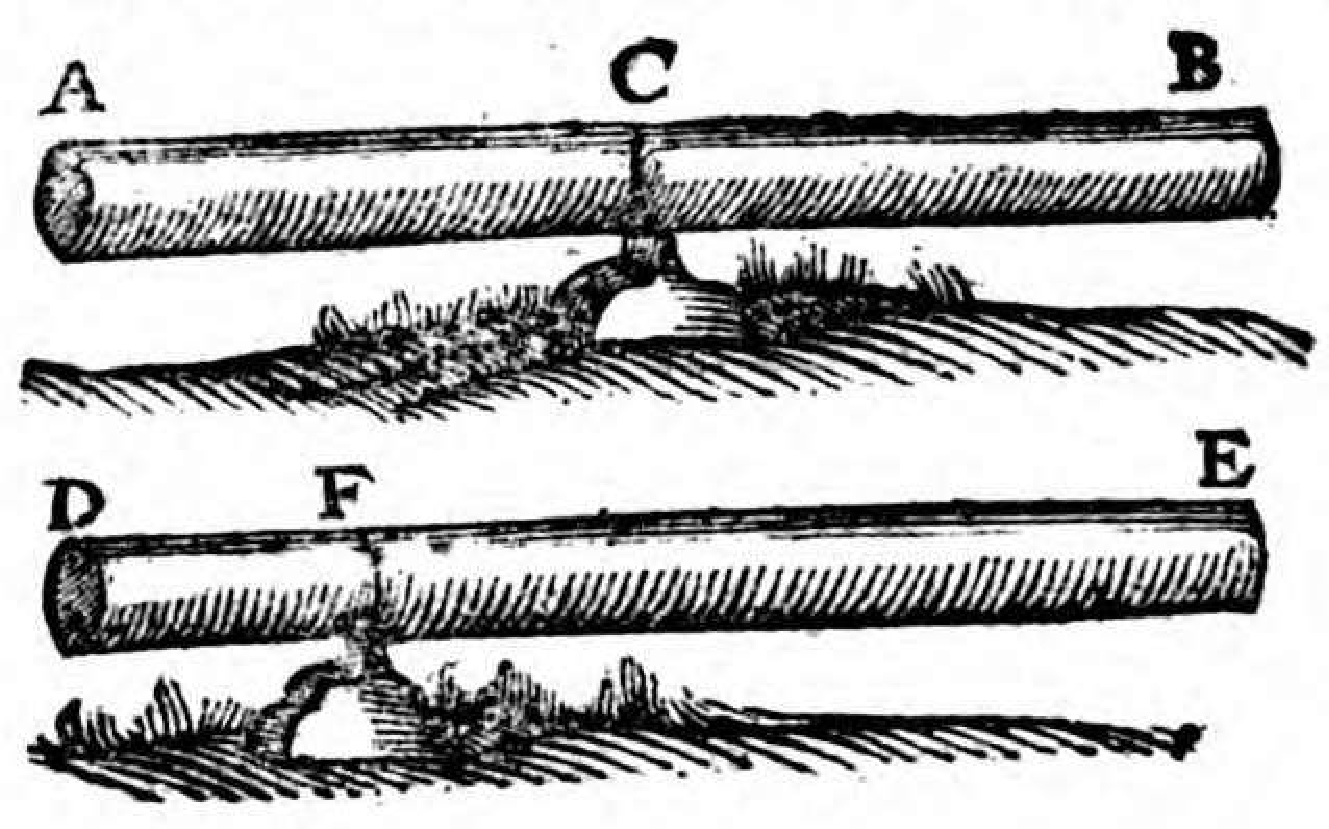
\includegraphics[width=0.5\textwidth]{images/Galilei_Opere_1556_Ausschn.pdf}\\
\rule{0mm}{10mm}\centering[\textit{Fig. 1; erg. Hrsg. nach Galilei}]\edtext{}{\lemma{\hspace*{1,8mm}[\textit{Fig. 1}]}\killnumber\Cfootnote{\cite{01084}Abbildung übernommen von G. \textsc{Galilei}, \textit{Discorsi}, Bologna 1656 (\textit{Opere}, Bd. II), S. 102 (\cite{00048}\textit{GO} VIII, S. 175). Zur Zeit seines Pariser Aufenthalts hat Leibniz diese Edition von Galileis \textit{Discorsi} gelesen. Siehe hierüber die Datierungsgründe in N. ??.% F/1 = 037,05_201
}}
%\caption{Bildbeschreibung}
% \end{center}
%\end{wrapfigure}
\pend
% \vspace*{1.5em}% PR: Rein provisorisch !!!
\newpage% Rein provisorisch !!!
\pstart%
\noindent%
\edlabel{37.05_202_1}\edtext{}{{\xxref{37.05_202_1}{37.05_202_2}}\lemma{Et per consequens [...] extremitatem $D$}\Cfootnote{Der nicht als gesperrt gedruckter Text ist die wörtliche lateinische Übersetzung einer Passage aus \cite{00050}G. \textsc{Galilei}, \textit{Discorsi}, Leiden 1638, S. 134f. (\textit{GO} VIII, S. 174f.\cite{00048}). Auf diese Passage nimmt Leibniz ausdrücklich in N. ?? % F/1 = 037,05_201
Bezug.}}%
Et per consequens opus est ipsum%
\textso{ (momentum}\protect\index{Sachverzeichnis}{momentum}%
\textso{ scilicet virium}\protect\index{Sachverzeichnis}{vis}%
\textso{ in \textit{D}\,) }%
crescere,%
\textso{ (in ea scilicet ratione, qua decrevit linea \textit{DF},
ut, si linea \textit{DF} sit dimidia lineae \textit{AC.}
pondus}\protect\index{Sachverzeichnis}{pondus}\textso{ in
\textit{D} fiat duplum ponderis incumbentis in \textit{A}\,) }%
ut aequare aut%
\textso{ (praecise, seu quantum satis est) }%
superare possit resistentiam\protect\index{Sachverzeichnis}{resistentia} in $F$%
\textso{ (supponit ergo resistentiam in $F$ absolute,
seu per se consideratam,
eandem esse quae fuit in $C$
quia requirit pondus $D$ tantum augeri
quantum distantia fuit diminuta,
ut proinde potentia}\protect\index{Sachverzeichnis}{potentia}\textso{ necessaria[,]
resistentiae scilicet aequivalens,
ac proinde et resistentia, maneat eadem.) }%
Sed distantia \textit{DF} diminui potest in infinitum, in relatione
ad distantiam \textit{AC.}
necesse est ergo posse crescere in infinitum vires applicandas in $D$
ad aequandam resistentiam\protect\index{Sachverzeichnis}{resistentia} in $F$%
\textso{ (verissime, nam si $F$ }%
\edtext{\textso{fulcrum}\protect\index{Sachverzeichnis}{fulcrum}}{\lemma{\textso{fulcrum}}\Bfootnote{\textit{ erg.} \textit{ L}}}%
\textso{ promoveri intelligatur usque sub ipsum $D.$
distantia \textit{DF} erit infinite parva,
ac proinde pondus appensum in $D$ debebit esse infinitum,
ut aequivaleat ponderi in $A$ incumbenti,
cumque non possit esse nisi finitum,
effectus}\protect\index{Sachverzeichnis}{effectus}%
\textso{ ejus erit infinities minor debito, seu 0. nullus.) }%
Sed contra, quatenus crescit distantia \textit{FE}
super distantiam \textit{CB.} convenit
diminui pondus\protect\index{Sachverzeichnis}{pondus}
seu potentiam\protect\index{Sachverzeichnis}{potentia} in $E$
ad aequandam resistentiam\protect\index{Sachverzeichnis}{resistentia} in $F$.
Sed distantia $FE$ in relatione ad $CB$ non potest crescere in infinitum,
utcunque fulcrum\protect\index{Sachverzeichnis}{fulcrum} $F$
a termino $E$ versus terminum $D$ removeatur,
imo nunquam excedere potest duplum
\edtext{distantiae}{\lemma{distantiae}\Bfootnote{\textit{ erg.} \textit{ L}}}
\textit{CB}.%
\textso{ (Certissime, nam si  $F$ maxime removeatur[,]
id est, usque sub $D.$ distantia \textit{FE} aequabitur lineae
\textit{DE}, id est \textit{AB} seu duplicatae \textit{CB}.) }%
\edtext{Ergo pondus\protect\index{Sachverzeichnis}{pondus}
seu potentia\protect\index{Sachverzeichnis}{potentia}}{\lemma{Ergo}\Bfootnote{ \textit{(1)}\ vis\protect\index{Sachverzeichnis}{vis} \textit{(2)}\ pondus seu potentia \textit{ L}}}
in $E.$ ut aequet resistentiam\protect\index{Sachverzeichnis}{resistentia} in $F.$
erit semper plus quam dimidium ponderis\protect\index{Sachverzeichnis}{pondus} applicati
\edtext{in $B.$%
\textso{ (Ita sane.}}{\lemma{in $B.$}\Bfootnote{\textit{ (1) }
% \lbrack \textit{Nachfolgend kleingedruckter Text in der Handschrift gestrichen:}\rbrack \footnotesize\
(Hic me attonitum fateor.
Cum omnia huc usque dicta sint verissima,
cum id quod nunc dicitur non tantum sit falsum,
et ex praemissis non inferatur,
sed et inferendum sit ejus contrarium
et quidem manifeste;
non possum capere
qui potuerit tale quiddam excidere tanto viro
quantus est omnium consensu Galilaeus.\protect\index{Namensregister}{\textso{Galilei} (Galilaeus, Galileus), Galileo 1564-1642}
% \normalsize
\textit{ (2) } \textso{(Ita sane} \textit{ L}}}%
\textso{ Nimirum, cum \textit{FE} nunquam, nisi fulcro}\protect\index{Sachverzeichnis}{fulcrum}\textso{ }%
\edtext{$F$}{\lemma{$F$}\Bfootnote{\textit{ erg.} \textit{ L}}}%
\textso{ plane opposito extremo }%
\edtext{$D$}{\lemma{$D$}\Bfootnote{\textit{ erg.} \textit{ L}}}%
\edtext{\textso{ supposito, contra}}{\lemma{\textso{supposito,}}\Bfootnote{ \textit{(1)}\ \textso{quod est contra hypothesin\protect\index{Sachverzeichnis}{hypothesis}, quod fulcrum\protect\index{Sachverzeichnis}{fulcrum} maneat} \textit{(2)}\ \textso{contra} \textit{ L}}}
\textso{hypothesin, fulcrum }%
\edtext{\textso{nempe}}{\lemma{\textso{nempe}}\Bfootnote{\textit{ erg.} \textit{ L}}}
\textso{ manere inter duo extrema, }%
\edtext{\textso{duplicetur, ad duplum}}{\lemma{\textso{duplicetur},}\Bfootnote{ \textit{(1)}\ \textso{dimidietur, nunqu} \textit{(2)}\ \textso{ad dimidium} \textit{(3)}\ \textso{ad duplum} \textit{ L}}}%
\textso{ usque decrescat;
potentia, ut eadem scilicet maneat quae }%
\edtext{\textso{prior, nunquam}}{\lemma{\textso{prior}}\Bfootnote{ \textit{(1)}\ \textso{in summa}  \textit{(2)}\ \textso{nunquam} \textit{ L}}}%
\textso{ ad dimidium usque minuetur,
seu semper erit dimidio major.) }%
% \pend
% \pstart
Ex his jam comprehendi potest,
\lbrack202~v\textsuperscript{o}\rbrack\
momenta seu momentum aggregati virium
in $E$ et $D$ augeri debere in infinitum ut
aequet aut superet resistentiam\protect\index{Sachverzeichnis}{resistentia} positam 
in $F$ prout fulcrum\protect\index{Sachverzeichnis}{fulcrum}
\edtext{$F$ accedet}{\lemma{$F$}\Bfootnote{ \textit{(1)}\ ibit \textit{(2)}\ accedet \textit{ L}}}
ad \edtext{extremitatem $D.$\edlabel{37.05_202_2}%
\newline%
\hspace*{7,5mm}%
Hic}{\lemma{}\Bfootnote{extremitatem $D.$\ \textbar\ ( \textit{streicht Hrsg.}\ \textbar\ Hic\ \textit{L}}}
me attonitum fateor,
cum omnia \edtext{toto fortasse tractatu,}{\lemma{toto fortasse tractatu}\Cfootnote{Gemeint sind Galileis \cite{00050}\textit{Discorsi}.}}
certe ea saltem, quae nunc recitavimus huc usque dicta
sint verissima[;]
cum id quod nunc dicitur
non tantum sit falsum nec ex praemissis inferendum,
sed et inferendis directe contrarium;
cum denique is qui dicat sit Galilaeus,\protect\index{Namensregister}{\textso{Galilei} (Galilaeus, Galileus), Galileo 1564-1642}
philosophus omnium consensu maximus;
aegre mihi ipsi credere
\edtext{potui}{\lemma{}\Bfootnote{potui \textit{ erg.} \textit{ L}}}, vel eum
\edtext{hoc scribere,}{\lemma{hoc}\Bfootnote{ \textit{(1)}\ dicere \textit{(2)}\ scribere \textit{ L}}}
vel cum scribat,
\edtext{errare; ad }{\lemma{errare;}\Bfootnote{ \textit{(1)}\ alterum \textit{(2)}\ ad \textit{ L}}}
fidem tamen alterius oculi, alterius
ratio mihi fecere. Quod scribat ex recitatis apparere arbitror, quod falsa sententia sit, ita ostendo.
\edtext{Si resistentia,\protect\index{Sachverzeichnis}{resistentia}}{\lemma{Si}\Bfootnote{ \textit{(1)}\ potentia\protect\index{Sachverzeichnis}{potentia} \textit{(2)}\ resistentia \textit{ L}}} 
seu vis ad frangendum necessaria
\edtext{applicanda in $D$ et $E$, conjunctim sumta}{\lemma{}\Bfootnote{applicanda in $D$ et $E$, conjunctim sumta \textit{ erg.} \textit{ L}}}, non dicam
in infinitum, sed vel
\edtext{tantillum ultra}{\lemma{tantillum}\Bfootnote{ \textit{(1)}\ crescit \textit{(2)}\ ultra \textit{ L}}} 
potentiam\protect\index{Sachverzeichnis}{potentia} in \textit{A} et \textit{B}, conjunctim sumtam,
\edtext{crescit, ob}{\lemma{crescit,}\Bfootnote{ \textit{(1)}\ crescet certe maxime  \textit{(2)}\ ob \textit{ L}}} 
fulcrum\protect\index{Sachverzeichnis}{fulcrum} $F$ 
\edtext{remotum a $C$ medio versus}{\lemma{remotum}\Bfootnote{ \textit{(1)}\ ab $E$ versus \textit{(2)}\  a $C$ medio versus  \textit{ L}}}
$D$ alterum extremorum, certe maxime crescet, quando fulcrum\protect\index{Sachverzeichnis}{fulcrum}
$F$ maxime remotum erit versus \textit{D} seu quando
statuetur sub ipso $D$[;] at quando statuetur fulcrum\protect\index{Sachverzeichnis}{fulcrum}
sub ipso $D.$ potentia\protect\index{Sachverzeichnis}{potentia} in $E$ erit praecise dupla
potentiae\protect\index{Sachverzeichnis}{potentia} in $B.$
Ergo id omne quod ponderi\protect\index{Sachverzeichnis}{pondus} $D$
\edtext{antea ipsi potentiae\protect\index{Sachverzeichnis}{potentia} aequali}{\lemma{}\Bfootnote{antea ipsi potentiae\protect\index{Sachverzeichnis}{potentia} aequali\textit{ erg.} \textit{ L}}}
ablatum, nihil enim nunc ponderat\protect\index{Sachverzeichnis}{pondus} fulcro\protect\index{Sachverzeichnis}{fulcrum}
$F$ ei supposito, id in pondus\protect\index{Sachverzeichnis}{pondus} $E$ translatum
est, aequat ergo resistentiam\protect\index{Sachverzeichnis}{resistentia} $F$, ut ante,
resistentia\protect\index{Sachverzeichnis}{resistentia} enim ipsa per se mansit eadem;
tantum an pondera\protect\index{Sachverzeichnis}{pondus} compensentur quaestio
est, quod hinc patet, cum in duobus sibi oppositis
statibus, cum fulcrum\protect\index{Sachverzeichnis}{fulcrum} est in medio, et cum est sub uno
\edtext{extremorum, eadem}{\lemma{extremorum,}\Bfootnote{ \textit{(1)}\ idem \textit{(2)}\ eadem \textit{ L}}}
nihilominus maneat potentia,\protect\index{Sachverzeichnis}{potentia} nihil addendo vel demendo,
sola mutua compensatione distantiarum.
\pend
\pstart
Idem absolute calculo quodam universali demonstrabimus,
ostendemusque propositionem quandam elegantem, nec hactenus observatam,
si de ipsorum Trabium\protect\index{Sachverzeichnis}{trabs} pondere\protect\index{Sachverzeichnis}{pondus} proprio ad
rupturam\protect\index{Sachverzeichnis}{ruptura} suffecturo quaeratur, tum vero
non augeri, sed contra minui resistentiam\protect\index{Sachverzeichnis}{resistentia},
fulcro\protect\index{Sachverzeichnis}{fulcrum} a medio discedente, nec brachiorum\protect\index{Sachverzeichnis}{brachium} vim utrinque compensari. Quae cum
sint adeo clara, ut partim ostendimus, partim
ostendemus, adeo contraria 
\edtext{Galilaeanis, ut ubi}{\lemma{Galilaeanis,}\Bfootnote{ \textit{(1)}\ adeo \textit{(2)}\ ut ubi \textit{ L}}} 
accidit resistentiae\protect\index{Sachverzeichnis}{resistentia} mutatio ob mutationem fulcri,\protect\index{Sachverzeichnis}{fulcrum} 
\edtext{contrarium eveniat}{\lemma{contrarium}\Bfootnote{ \textit{(1)}\ accidat \textit{(2)}\ eveniat \textit{ L}}} 
ejus pronunciato, minuatur scilicet, non augeatur resistentia.\protect\index{Sachverzeichnis}{resistentia}
Id nobis documento esse debet nihil etiam
a summis viris dictum, sine exacta discussione,
\lbrack203~r\textsuperscript{o}\rbrack\
pro principio demonstrationis assumendum esse;
quod tamen non paucos in hoc argumento fecisse
video.
\pend
\pstart
Auget\edlabel{37.05_203r_a1} vero admirationem meam
quod \edtext{Galilaeus\protect\index{Namensregister}{\textso{Galilei} (Galilaeus, Galileus), Galileo 1564-1642}
huic ipsi ratiocinationi ea omnia superaedificat 
\edtext{quae de figuris}{\lemma{quae}\Bfootnote{ \textit{(1)}\ figurarum \textit{(2)}\ de figuris \textit{ L}}} 
trabium\protect\index{Sachverzeichnis}{trabs} ad sustinenda onera\protect\index{Sachverzeichnis}{onus} aptissimarum, quo ille Elogio prae caeteris
parabolam donat, ratiocinatur.}{\lemma{Galilaeus [...] ratiocinatur}\Cfootnote{\cite{00050}G. \textsc{Galilei}, \textit{Discorsi}, Leiden 1638, S. 137-141 (\textit{GO} VIII, S. 177-181).\cite{00048}}}
Et vero rectissime nuper animadversum est
\edtext{ab egregio viro,}{\lemma{ab egregio viro}\Cfootnote{Quelle nicht nachgewiesen.}}
parabolam spei non respondere,
attamen ratiocinatio Galilaei\protect\index{Namensregister}{\textso{Galilei} (Galilaeus, Galileus), Galileo 1564-1642}
adeo ab eo excussa non est,
ut etiam quibus\-dam ejus principiis
\edtext{quae}{\lemma{}\Bfootnote{quae \textit{ gestr. L, wieder gültig gemacht Hrsg.}}}
\edtext{nunc examinabimus,}{\lemma{nunc}\Bfootnote{ \textit{(1)}\ examinamus \textit{(2)}\ examinabimus \textit{ L}}}
usus sit,
unde fons erroris huc usque indetectus \edlabel{37.05_203r_a2}mansit.
\pend
\pstart
Caeterum adeo sibi placet in praesenti ratiocinatione Galilaeus\protect\index{Namensregister}{\textso{Galilei} (Galilaeus, Galileus), Galileo 1564-1642}
ut \edtext{collocutores faciat exclamare,
prae admiratione subtilitatis, et attolere vim Geometriae,
quae res scilicet tam a prima specie remotas,
protrahat in lucem.}{\lemma{collocutores [...] in lucem}\Cfootnote{\cite{00050}G. \textsc{Galilei}, \textit{Discorsi}, Leiden 1638, S. 135 (\textit{GO} VIII, S. 175).\cite{00048}}}
Et vero hoc jam fundamento structo,
quod resistentia\protect\index{Sachverzeichnis}{resistentia} augeatur,
fulcro\protect\index{Sachverzeichnis}{fulcrum} magis a medio remoto,
\edtext{conatur investigare augmenti proportionem.}{\lemma{conatur [...] proportionem}\Cfootnote{\cite{00050}a.a.O., S. 135f. (\textit{GO} VIII, S. 176).\cite{00048}}}
\pend
\pstart
Quod antequam persequamur,
dicendum est, quid videatur duxisse tantum virum,
aliis fortasse cogitationibus, ut solemus homines, non aeque semper
nobis esse praesentes, distractum.
Videtur ita ratiocinari voluisse:
manifestum est potentiam\protect\index{Sachverzeichnis}{potentia} ex $A$ in $D$ minui in infinitum,
quia \edtext{[\textit{DF}]}{\lemma{\textit{DC}}\Bfootnote{ \textit{L ändert Hrsg.}}}
potest esse $\displaystyle\frac{1}{2}$ vel $\displaystyle\frac{1}{3}$ vel $\displaystyle\frac{1}{4}$ etc.
de \textit{AC}. Necesse est ergo et potentiam\protect\index{Sachverzeichnis}{potentia} ex $B$ in $E$
augeri in infinitum, ut compensatione facta summa
\edtext{duarum}{\lemma{}\Bfootnote{duarum \textit{ erg.} \textit{ L}}} 
potentiarum,\protect\index{Sachverzeichnis}{potentia}
\edtext{ut ante, resistentiae\protect\index{Sachverzeichnis}{resistentia}}{\lemma{ut ante,}\Bfootnote{ \textit{(1)}\ potentiae \textit{(2)}\ resistentiae \textit{ L}}} 
in $C$ vel $F$ quae per se eadem manet, aequiponderet. At vero
non potest potentia\protect\index{Sachverzeichnis}{potentia} in $E$ ex $B$ sola remotione
fulcri\protect\index{Sachverzeichnis}{fulcrum} ab $E$ versus
\edtext{[$D$]}{\lemma{$B$}\Bfootnote{\textit{ L ändert Hrsg.}}}
augeri in infinitum,
cum etiam maxima fulcri\protect\index{Sachverzeichnis}{fulcrum} remotione, usque ad $D$
non nisi duplicetur; cum ergo
\edtext{distantia potentiae\protect\index{Sachverzeichnis}{potentia} $E$ a fulcro\protect\index{Sachverzeichnis}{fulcrum} $F$ seu magnitudo brachii\protect\index{Sachverzeichnis}{brachium}}{\lemma{distantia}\Bfootnote{\textbar\ potentiae $E$ a fulcro\protect\index{Sachverzeichnis}{fulcrum} $F$ \textit{ erg.} \textbar\  \textit{ (1)}\ brachii \textit{ (2)}\ seu magnitudo brachii \textit{ L}}}
$FE$ ultra 
\edtext{$CB$ aucta fulcro\protect\index{Sachverzeichnis}{fulcrum} in ipsum usque $D$ utcunque, ac proinde non nisi finite remoto}{\lemma{$CB$}\Bfootnote{ \textit{ (1)}\ ac proinde non aucta nisi finite \textit{ (2)}\ utcunque \textit{ (3)}\ remoto fulcro in ipsum usque $D$ utcunque, ac proinde non nisi finite aucta  \textit{ (4)}\  aucta [...] remoto \textit{ L}}}[,]
non compenset in potentia\protect\index{Sachverzeichnis}{potentia} $E$
\edtext{quantum perdi potest}{\lemma{quantum}\Bfootnote{ \textit{(1)}\ perditum est \textit{(2)}\ perdi potest \textit{ L}}}
in potentia $D$
\edtext{quippe}{\lemma{}\Bfootnote{quippe \textit{ erg.} \textit{ L}}}
in infinitum diminuibili ob distantiam infinities diminuibilem,
manifestum est, ad compensationem faciendam,
necesse esse pondera\protect\index{Sachverzeichnis}{pondus} augeri, ac per consequens
\edtext{resistentiam\protect\index{Sachverzeichnis}{resistentia} ex $C$ in $F$}{\lemma{resistentiam}\Bfootnote{ \textit{(1)}\ in $C$ vel $F$ \textit{(2)}\ ex $C$ in $F$ \textit{ L}}}
non quidem per se sed ob ponderum\protect\index{Sachverzeichnis}{pondus} situm, esse auctam.
\pend
\pstart
Speciosus sane paralogismus,
qui potissimum in hoc consistit,
quod Galilaeus\protect\index{Namensregister}{\textso{Galilei} (Galilaeus, Galileus), Galileo 1564-1642}
augmentum et diminutionem brachiorum\protect\index{Sachverzeichnis}{brachium} assumsit,
ut multiplicationem et divisionem,
non vero ut additionem et subtractionem.
Nam si additio et subtractio
\lbrack203~v\textsuperscript{o}\rbrack\
abhibeantur, manifestum est quantum uni brachio\protect\index{Sachverzeichnis}{brachium} decedit,
tantum alteri accedere.
Unde ad compensationem
faciendam, non est necesse si unum dimidiatur, alterum
duplicari, ut sunto duae
\edtext{summae, aequales}{\lemma{summae,}\Bfootnote{ \textit{(1)}\ altera \textit{(2)}\ aequales \textit{ L}}} 
v.g. $4+4=8$. Si jam uno diminuto alterum
augere velis, ita ut summa uti ante maneat 8.
non per viam
\edtext{multiplicationis et divisionis sed }{\lemma{multiplicationis}\Bfootnote{ \textit{(1)}\ sed \textit{(2)}\ et divisionis sed  \textit{ L}}} 
additionis et subtractionis procedendum est[,] uti si
\edtext{unum}{\lemma{}\Bfootnote{unum \textit{ erg.} \textit{ L}}}
4 dimidies habebis 2. Non ideo duplicandus est
alter 4narius, ita enim habebis $8+2=$ non 8 sed 10.
Et ratio est, quia ut summa eadem maneat
postulatur, non ut factus duorum numerorum inter se,
si factum esse eundem postuletur, fateor, quantum 
\edtext{unus minuitur,}{\lemma{unus}\Bfootnote{ \textit{(1)}\ dividitur \textit{(2)}\ minuitur \textit{ L}}}
tantum alterum esse multiplicandum, ut 
$4\smallfrown4=16.$ $\displaystyle\frac{4}{2}\smallfrown4\smallfrown2=2\smallfrown8=16.$
Quare una potentia\protect\index{Sachverzeichnis}{potentia} $D$ ex $A$ dimidiata[,]
Brachio\protect\index{Sachverzeichnis}{brachium} scilicet \textit{DF} ex \textit{AF} dimidiato[,] non est
necesse (imo necesse est non) duplicari
\edtext{alteram}{\lemma{}\Bfootnote{alteram \textit{ erg.} \textit{ L}}}
potentiam\protect\index{Sachverzeichnis}{potentia} $E$ ex $B.$ vel brachium \textit{FE} ex \textit{CB.}
\edtext{sed}{\lemma{}\Bfootnote{sed \textit{ erg.} \textit{ L}}} 
sufficit (imo necesse est) ei addi potentiam\protect\index{Sachverzeichnis}{potentia} seu distantiam alteri ademtam,
quod ipsa fulcr\protect\index{Sachverzeichnis}{fulcrum}i translatione jam contigit.
Esto enim ut res exemplo pateat pondus\protect\index{Sachverzeichnis}{pondus}
\edtext{rupturae\protect\index{Sachverzeichnis}{ruptura} in $C$ sufficiens}{\lemma{}\Bfootnote{rupturae\protect\index{Sachverzeichnis}{ruptura} in $C$ sufficiens \textit{ erg.} \textit{ L}}} 
tam in $A$ quam in
\edtext{$B$ unumquodque}{\lemma{$B$}\Bfootnote{ \textit{(1)}\ utrumque \textit{(2)}\ unumquodque \textit{ L}}} 
8. totum 16 librarum;
\edtext{nam}{\lemma{}\Bfootnote{nam \textit{ erg.} \textit{ L}}}
dimidiato brachio\protect\index{Sachverzeichnis}{brachium} \textit{EF} ex \textit{AC} fiet
potentia\protect\index{Sachverzeichnis}{potentia} $D$ ex $A$ dimidiata, librarum 4. Quod si
\edtext{alteram $E$ ex $B$ duplicato}{\lemma{alteram}\Bfootnote{ \textit{(1)}\ duplicamus \textit{(2)}\ $E$ ex $B$ duplicato  \textit{ L}}}
brachio,\protect\index{Sachverzeichnis}{brachium} vel potius cum id ob fulcrum\protect\index{Sachverzeichnis}{fulcrum} in $F$ medium \textit{AC}
remotum non contingat, duplicato pondere\protect\index{Sachverzeichnis}{pondus}
appenso, itidem duplicare velimus, fiet librarum
16. et summa librarum 20. cum debeat esse
non nisi 16. At si simpliciter distantiam alteri
potentiae\protect\index{Sachverzeichnis}{potentia} ademtam, alteri addas, uti fulcro\protect\index{Sachverzeichnis}{fulcrum} moto
per se contingit, calculus semper respondebit: ut hoc
\edtext{loco dimidium abstulimus brachio\protect\index{Sachverzeichnis}{brachium}}{\lemma{loco}\Bfootnote{ \textit{(1)}\ brachii \textit{(2)}\ dimidium abstulimus brachio \textit{ L}}}
\textit{AC} translato fulcro\protect\index{Sachverzeichnis}{fulcrum} in $F$ id dimidium
\edtext{brachii\protect\index{Sachverzeichnis}{brachium} nempe}{\lemma{brachii}\Bfootnote{ \textit{(1)}\ \textit{AC} a  \textit{(2)}\ nempe \textit{ L}}} 
\textit{FC} addemus brachio\protect\index{Sachverzeichnis}{brachium} \textit{CB} et
fiet \textit{FE}. Jam brachium\protect\index{Sachverzeichnis}{brachium} \textit{FE} est sesquialterum
brachii \textit{CB} seu est ad ipsum ut 3 ad 2.
Ergo et potentia\protect\index{Sachverzeichnis}{potentia} in $D$ eo ipso potentiae\protect\index{Sachverzeichnis}{potentia} in $B$
sesquialtera est, seu cum potentia\protect\index{Sachverzeichnis}{potentia} in $B$ fuerit
8. potentia in $D$ fiet 12.
$\displaystyle \left(8\smallfrown \frac{3}{2} = \frac{24}{2} =12 \right).$
Jam $\displaystyle 12 + 4 = 16$ ut ante. Et vero nunquam
fiet, ut duabus quantitatibus altera duplicata  
altera vero dimidiata, summa productorum
eadem sit quae ante quantitatum, nisi dimidiata
ante dimidiationem fuerit dupla duplicatae
ante duplicationem. Statuemus autem infra
regulam\protect\index{Sachverzeichnis}{regula generalis}
\edtext{generalem, de}{\lemma{}\Bfootnote{generalem, \ \textbar \ \ per quam agnosci queat \textit{ gestr.}\ \textbar\ de \textit{ L}}}
eo scilicet casu, in quo solo contingit duabus
quantitatibus altera in eadem ratione aucta,
in qua altera est minuta, summam productorum,
aequari summae quantitatum.
\pend

%
%Glossar:
%brachium
% pondus
%onus
% resistentia
% potentia
% fulcrum
% effectus
% trabs
% ruptura
% regula generalis
%Galilei
%hypothesis